\section{Dynamic Agents in MATSim}
\label{sec:dynagent}

Several approaches have been proposed to allow for dynamic behavior in MATSim.
The decision on which option is best depends mainly on what a
level of complexity in the behavior is needed.

A simple version of dynamic behavior is implemented in the public transport (PT)
extension, where passenger agents are saved in a list as soon as they reach the
link in the network, where they should be picked up by a public transport agent.
As soon as the PT agent (e.g. a bus) arrives at that link, persons from the link
are deregistered from the list and ``teleported'' to the destination stop as soon
as the vehicle arrives there. This setup fits very well into the queue based structure
of MATSim.

An even more dynamic approach is used in the DVRP framework, which will be discussed
in the first part of this section. At the time of this thesis and for the specific
use case of autonomous vehicles, some drawbacks will be shown and finally a new
abstraction layer for dynamically acting agents will be presented, which has been
part of the thesis work.

\subsection{DVRP}

The DVRP extension \citep{DVRP12, Horni2015} is designed to provide a level of abstraction to the simulation of
dynamic transport services, such as taxis. Its general structure is quite flexible
so that it is easy to implement for instance electric vehicles \citep{Bischoff2014} (which need to recharge
at some point during the simulation) or taxis, which are roaming randomly through
the city and serving requests when they are made by passengers \citep{Maciejewski2015}.

However, this flexibility comes at a cost: The architecture of DVRP
circumvents the efficient queue simulation of MATSim for activities. While ``normal''
agents are simulated as described before, dynamic agents (DynAgents) have two
modifications:

\begin{description}
\item[Legs] are sent to the conventional Netsim. However, agents have the ability
to change their paths dynamically, i.e. one can modify the route of the agent
during the simulation steps and the next time the Netsim wants to move the agent
or checks whether the agent should arrive at the current link, its response is
calculated from the updated path.
\item[Activities] are simulated separately from the non-dynamic agents. As soon
as a DynAgent starts an activity it is added to a list of active agents. In each
simulation step a specific callback for each of those agents is called and then
it is checked whether the agent wants to end this activity or not.
This polling approach, as depicted in \cref{fig:polling}, makes sure that it is
not necessary to know when an activity (for instance a taxi waiting for any
requests) should end or how long it should take. On the other hand, this approach
is much more computationally expensive than the efficient queue simulation.
Given that the simulation is done on a second-by-second basis, an activity that
would take one hour, would cost only one insert and one lookup on the acitivty queue.
In the polling approach it costs 3600 calls to the simulation step callback (even
if it does not actually compute anything, this adds a computational overhead) and
3600 checks whether the activity should be ended.
\end{description}

Using DVRP, \citet{Bischoff2016} ran a study
on autonomous vehicles, where the demand in Berlin has been
obtained using an ordinary MATSim simulation. Then the link speeds of the underlying
network have been modified, to resemble the traffic situation in a congested
situation and then \textit{only} autonomous vehicles have been simulated. This
means that the simulation could be run once, and the results were obtained because
only the QSim was used and not the evolutionary learning of MATSim.

However, in the project of this thesis, autonomous vehicles should be tested in
an existing multi-modal scenario, where the evolutionary learning is necessary
for the agents to arrive at their quasi-optimal mode choices. So if
\citet{Bischoff2016} mentions computational times of 20h for a large number of agents,
it is a measure for one iteration of the evolutionary algorithm. For the scenarios
that will be tested here, iterations still do not reach a satisfactory
equilibrium, although having a theoretical computation time of 2000h already.

Measurements have been made to determine, how much the simulation of an idle agent,
which always stays in one activity, would cost regarding execution time
on a test machine\footnote{Intel(R) Core(TM) i7-3612QM CPU @ 2.10GHz}. The final results
gave an average time of 25ns. So simulating for instance 8000 agents for a common
simulation time of 30h, would lead to an execution time of:

\begin{equation}
T_{30h} = \underbrace{25}_{\text{Nomial}} \cdot \underbrace{3600 \cdot 30}_{\text{One day in seconds}} \cdot \underbrace{8000}_{\text{Agents}} = 21.6s
\end{equation}

For the whole MATSim simulation, this needs to be multiplied by at least 100 iterations,
so that the overhead of a simulation of 8000 agents doing nothing would already
reach a (highly optimistic) computational overhead of

\begin{equation}
T_{sim} = 21.6s \cdot 100 = 36min
\end{equation}

Furthermore, while working with DVRP, it has been found that one needs to put
increased efforts into making the framework compatible with parallelized computation
in the Netsim, which would have lead to a neglect of a good way to improve the computational
performance of the simulation if ignored.

As a summary, one can say, that DVRP allows for a great freedom in simulating
dynamic behavior and its structure and signaling flows are very straight-forward
and easy to work with. However, for large numbers of iterations, it would
be beneficial to find more efficient ways for the simulation.

\begin{figure}
    \centering
    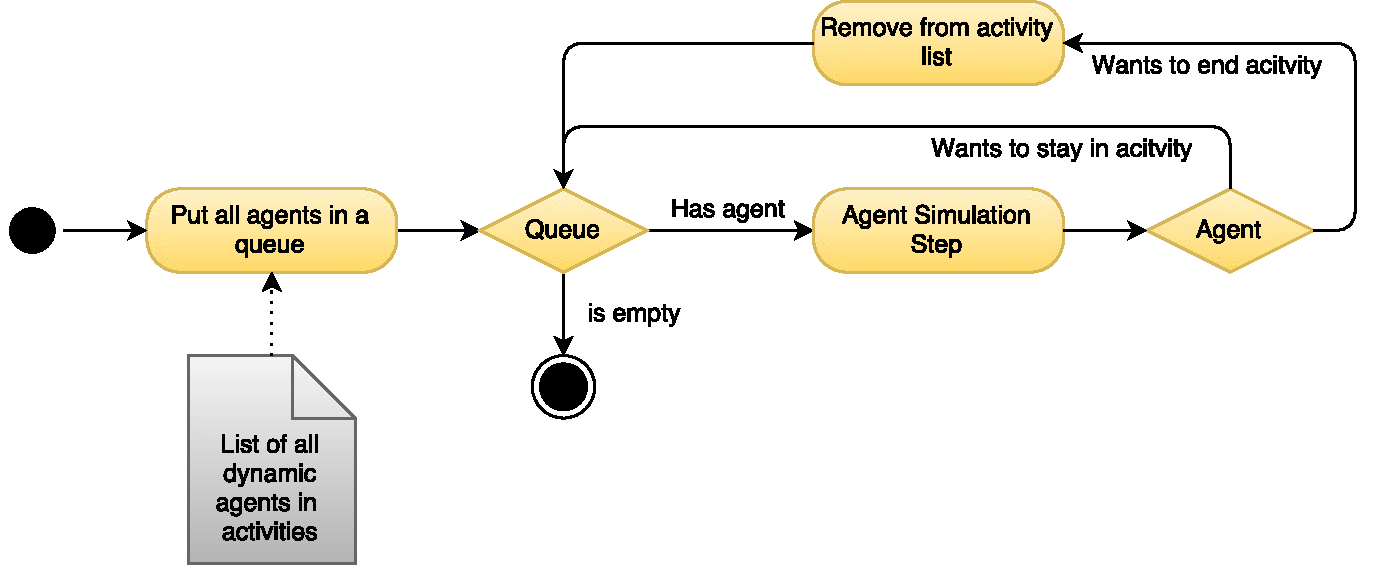
\includegraphics[width=1.0\textwidth]{figures/polling.pdf}
    \caption{Polling approach of the DVRP framework}
    \label{fig:polling}
\end{figure}

\subsection{The AgentLock framework}

As an alternative to the simulation of dynamic agents using DVRP, the AgentLock
framework has been developed as part of this thesis. It tries to combine the advantages
of a queue simulation while providing as much flexibility as possible to create
rich and dynamic agent behaviors in MATSim.

The basic idea is as follows: Usually agents in MATSim do not need much processing
power, i.e. the per-agent simulation step of DVRP is hardly ever used and can usually
replaced by some callbacks and event handlers outside of the actual agent simulation.

Furthermore, this means that an activity just means that an agent is residing
at a certain position in the network and not taking part of the network. So an
activity for an agent is just keeping the agent back from joining the traffic network
again after a certain time or event.

With this idea in mind, three different types of ways to ``lock'' an agent into
an activity have been proposed:

\begin{description}
    \item[Blocking] activities will just let the agent reside in this activity until
    it is released through a call from outside.
    \item[Time-based] activites are the ones from the basic MATSim simulation: They
    have a certain duration and therefore a fixed end time.
    \item[Event-based] activities let the agent reside in the activity until a certain
    event happens.
\end{description}

The heart of the AgentLock extension is the LockEngine. Whenever it encounters an
agent that wants to start a blocking or event-based activity, it is removed from
the simulation and only added back manually or as soon as the
event occurs. Then it either is passed to the ordinary Netsim or the next activity
is started, just as requested by the agent logic.

For time-based activities, a similar approach to the activity queue for ordinary
agents is taken. The first idea that would come to one's mind is to order the
agents by the end time of their activity and as soon as there is a change in plans,
remove the element from the priority queue and add it back at a certain position.

Compared to DVRP, where a change of plans would cost nothing, here this would lead
to an overhead of $\mathcal{O}(\log n)$ and $\mathcal{O}(n)$ for these operations \citep{JavaPQ}.
So it is necessary to weigh the overhead of the polling in DVRP against the overhead
of the rescheduling, which mainly depends on how often such reschedulings appear. In
the concrete example of autonomous taxis, this itself depends directly on the travel
demand.

If one sacrifices a slightly increased memory consumption for the sake of having a faster
computation time, this setup can be improved further, as done for the AgentLock
framework. Here, every time a time-based activity is started, a handle to the
corresponding agent is saved into the priority queue, ordered by the end time of
that activity. Furthermore, an indicator is saved, whether the handle is still valid.
So if in the meantime the plan is changed (i.e. before the end of the activity has been processed),
this handle will be invalidated, and it will simply be ignored when processing the priority queue.

The whole process (\cref{fig:lockengine}) works as follows: In every simulation step, the top element of
the priority queue is checked. If the top lock handle is scheduled for the current or a past time
step, the associated agent is saved for further processing. If the handle already had been invalidated, the processing continues with the
updated top element of the priority queue until a handle is found that has an expiry
time which lies in the future. Subsequently, the new state (activity or leg) is
computed for each saved agent, and a new lock handle is added to the handle queue if it
is time-based.

\begin{figure}
    \centering
    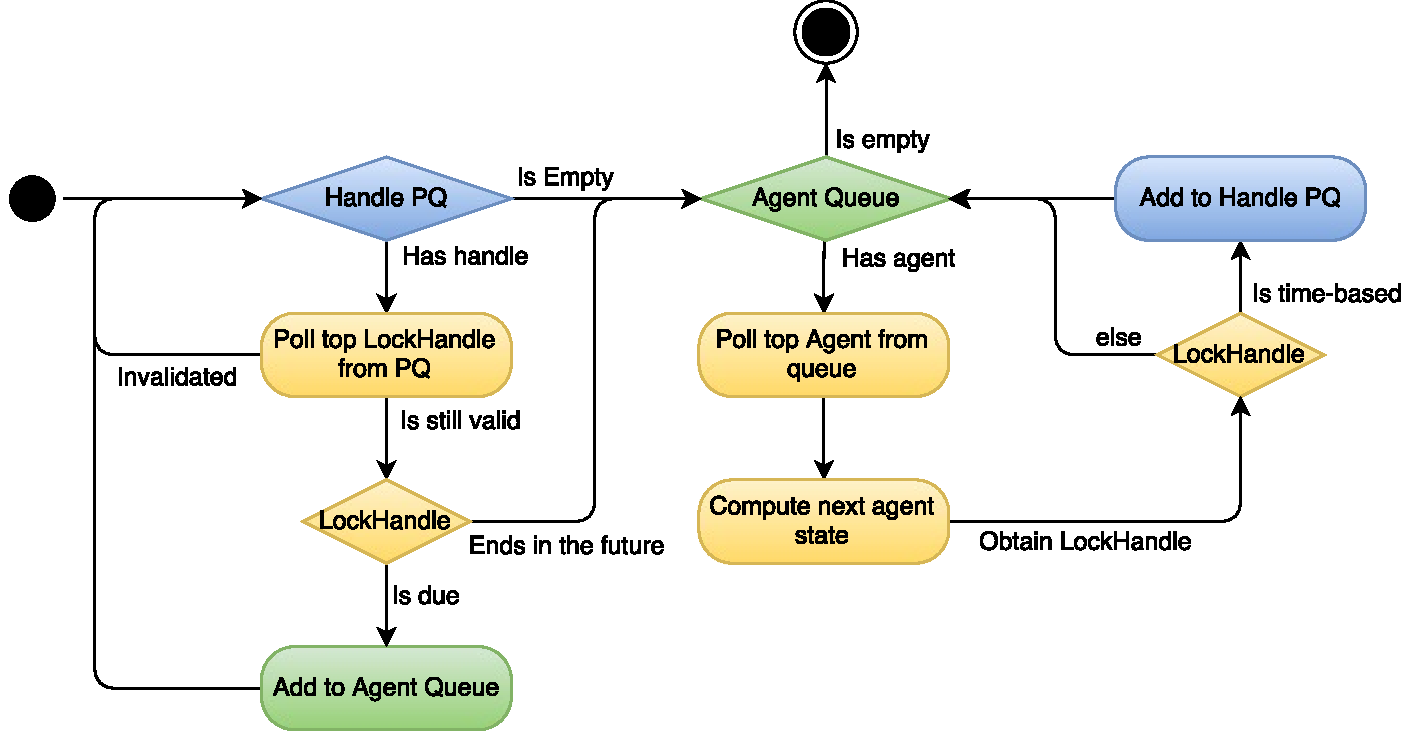
\includegraphics[width=1.0\textwidth]{figures/lockengine.pdf}
    \caption{Per-Iteration procedure of the LockEngine in the AgentLock framework}
    \label{fig:lockengine}
\end{figure}

The main advantage of this setup is that elements are only removed at the top
of the queue, which is significantly less expensive than removing elements at
arbitrary positions within the queue.

Furthermore, the AgentLock framework provides methods for dynamically ending legs,
and it has been made sure that all the functionality has a high degree of compatibility
with the existing parts of MATSim, such as the multi-threaded Netsim.

\subsection{AgentFSM}

While the AgentLock extension mainly provides an abstraction layer for the dynamic
rescheduling of activities and legs, another layer has been developed, which is
loosely resembling a finite state machine, tailored towards agents in
MATSim.

In this framework all the activities and legs are predefined states in a finite
state machine and the transitions from one step to another can either be triggered
manually (which is the \textit{blocking} lock from above), by time (\textit{time-base lock})
or by an event (\textit{event-based lock}).

The main task of the AgentFSM framework is to encapsulate common programming steps
when designing dynamic behavior in MATSim. This means that one usually just has
to define which states the behavior is built of and how the transition from one
to another works. All of this functionality is provided with a simple programming
interface.

In more detail, each state is either a LegState or an ActivityState. For each state,
an \textit{enter} callback exists, which the programmer can use to execute arbitrary
code. It needs to either return how this state is locked from the three options above or
issue a direct switch to another state.

As soon as the state is ended due to the above conditions, the \textit{leave} callback
of a state is called, which must return to which next state the simulation should
switch.

The concrete implementation for the autonomous vehicles will be discussed in \cref{sec:avmodel}.

\subsection{Comparison}

An implementation of autonomous vehicles in DVRP has been compared to an implementation
using the AgentLock framework. A specific number $n$ of
autonomous vehicles are created and put into a queue. As soon as an agent wants to
start a leg using an AV, the top element of the queue will drive to that position,
pick up the passenger, bring him to the final destination and drop him off. Then
the AV will be added back to the end of the queue. This dispatching algorithm is
quite inefficient but sufficient to do investigations in terms
of computation time for the two implementations since the behavior is equal and
easily understandable.

Simulations with $n=2000, 4000, 8000$ have been done on the Sioux-14 scenario. What can be seen in \cref{fig:dvrpfsm}
is the number AV legs in the simulation and the associated computation
time. For a large range, the implementation using AgentLock/AgentFSM (solid)
is much faster than the corresponding DVRP implementation (dashed). In fact, for $n=8000$
only at a (quite unrealistically big) AV share of around 60\%, DVRP starts to be more efficient.

Important to notice is that the performance of DVRP stays roughly the same over
the whole range of shares. This is because all 8000 AVs are simulated
in every single time-step, no matter if they are active or not. In the AgentLock
implementation, however, agents are only simulated if they are really in use. At
$110k$ legs, though, when the reschedulings of used AVs are getting too frequent, the repeated
queue operations get more expensive than the polling and therefore DVRP becomes more efficient.

As a result, one can say that the AgentLock implementation is usually more efficient
than the DVRP version if there is a limited number of reschedulings. If they get
too frequent, i.e. the behavior is characterized by many alterations of some
initial plan, the polling structure of DVRP gets more efficient. For the purpose
of simulating autonomous taxis in this thesis, the number of such reschedulings
should be minimal, as it will be described in \cref{sec:avmodel}. Therefore, the
development of the AgentLock framework indeed bears a computational advantage for
this thesis.

\begin{figure}
    \centering
    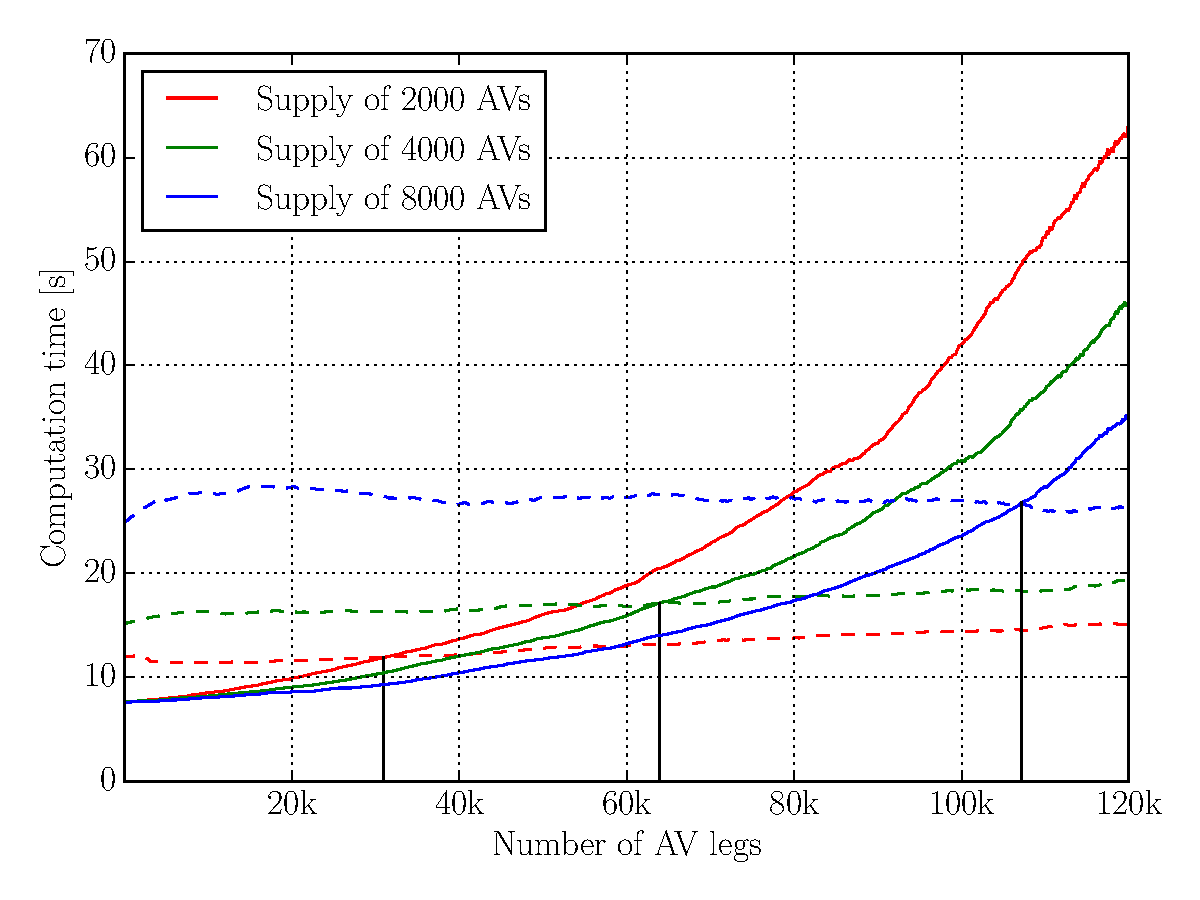
\includegraphics[width=0.7\textwidth]{figures/dvrp_fsm.pdf}
    \caption{Comparison of Mobsim runtimes between DVRP (dashed) and AgentLock/AgentFSM (solid) implementation, dependent on the number of AV legs. The scenario is Sioux-14 with
    a total number of legs of around 180k.}
    \label{fig:dvrpfsm}
\end{figure}

Regarding a multithreaded Mobsim, only tests with the new AgentLock implementation
could be done, as shown in \cref{fig:threads}. Obviously, though the improvement
is small, the simulation with two threads performed best. This shows that it is
an advantage to be able to use the multithreaded Mobsim. Similar results
have been found for other scenarios. For instance, the optimal number of threads
for the Singapore scenario has been found to be four \citep{Erath2014}.

\begin{figure}
    \centering
    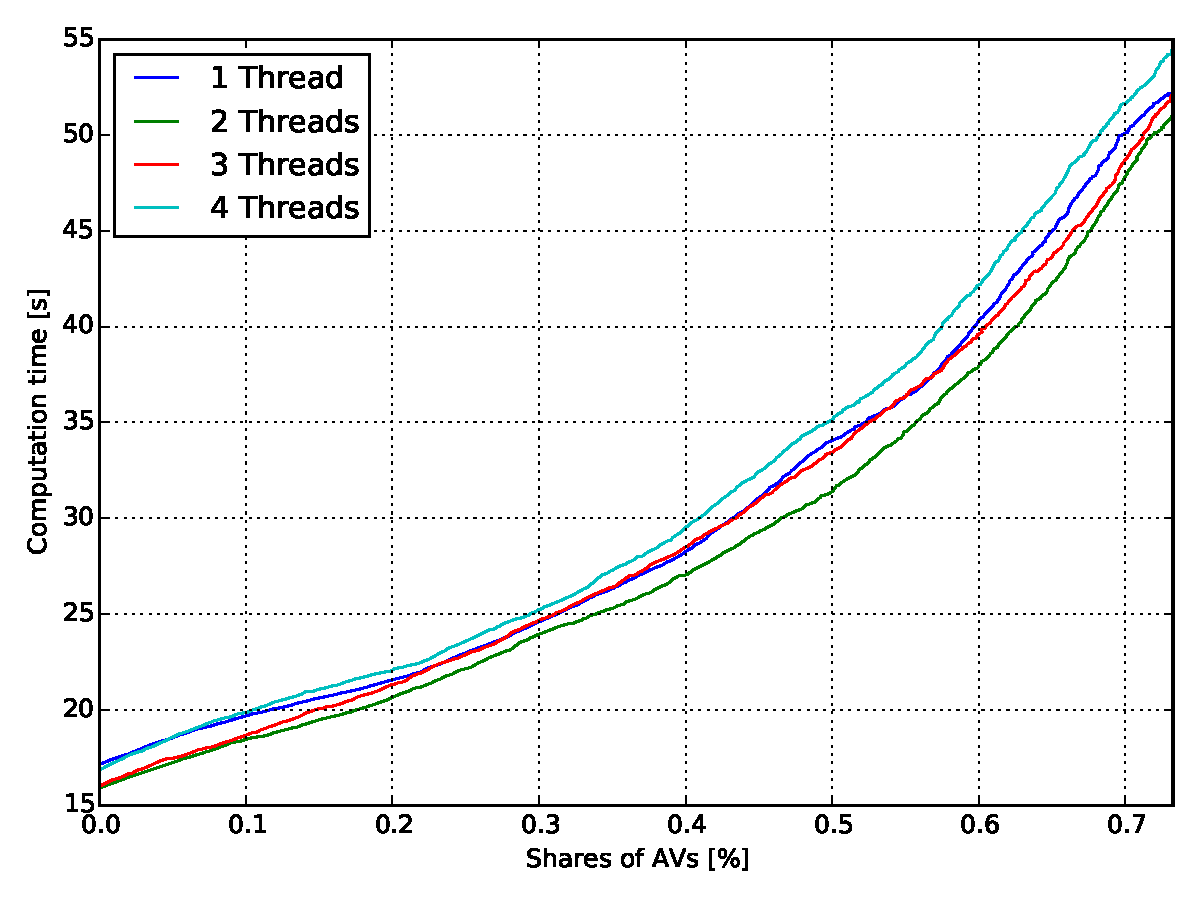
\includegraphics[width=0.7\textwidth]{figures/threads.pdf}
    \caption{Comparison of different numbers of threads for the Mobsim with the AgentLock implementation}
    \label{fig:threads}
\end{figure}

In conclusion, while the AgentLock framework is suited for the investigations in
this thesis, a hybrid framework, offering both approaches, would be highly beneficial.
While the AgentLock framework could be extended easily to provide this functionality,
another idea would be to integrate the locking approach into DVRP to create
a unified basis for dynamic agents in MATSim. Even more, it would be interesting
to investigate adaptive algorithms, which could switch intelligently between the
processing modes, dependent on the actual computation time and number of reschedulings
in a specific simulation.
